\chapter{序論}
\label{chapter:intro}

\pagenumbering{arabic}

書いたプログラムが思った通りの挙動をしない時、プログラマはデバッグをする必要がある。

単純なデバッグはプログラムを実行した際の出力から推測したりソースコードを眺めることで行われるが、そのようなデバッグは「ソースコードのどの部分が間違っているか」を示すものが無く、多くの時間や労力を要することがある。特にプログラミングにまだ慣れていない初学者にとっては、デバッグの経験や言語に対する理解が乏しい為、より困難な作業になると考えられる。

そこで色々な言語にデバッガが用意されているが、デバッガを利用するには、デバッガのコマンドの文字列や意味を覚えたり、ブレイクポイントを設定する箇所を考えたりといった、初学者にとってやはり困難な操作が必要になる。また、一般的なデバッガで表示されるのは「ソースコード中の実行中の行」であり、どこで今の関数を呼び出されたのか、この後どんな計算があるのかなどといったプログラム全体の流れが分かりにくい。

\begin{figure}
  \begin{center}
    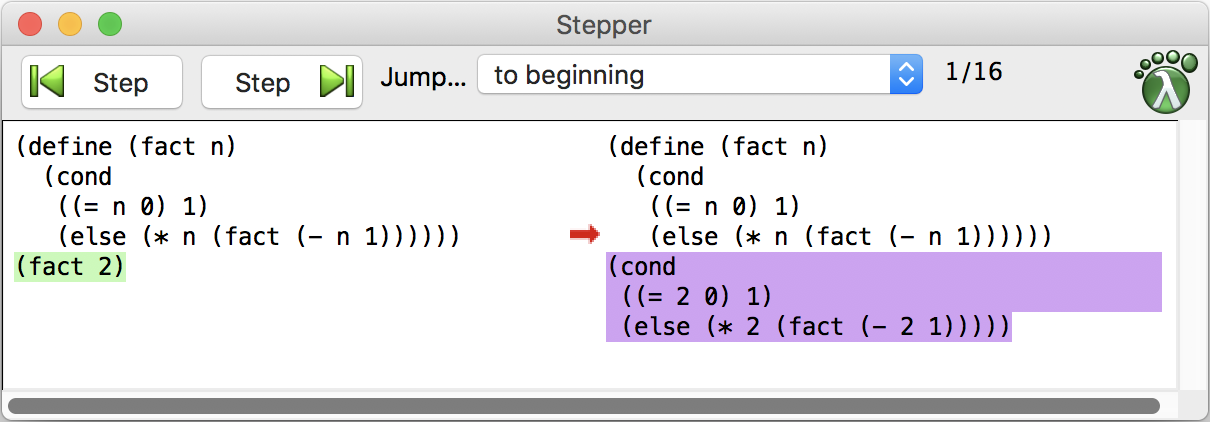
\includegraphics[width=13cm]{1/racket1.png}
  \end{center}
  \caption{DrRacket のステッパ}
  \label{figure:racket1}
\end{figure}

\begin{figure}
  \begin{center}
    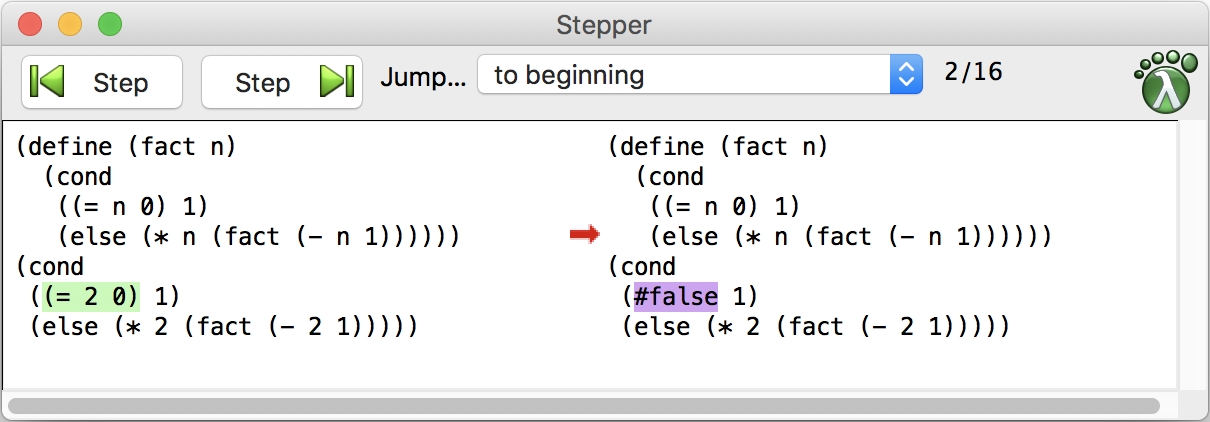
\includegraphics[width=13cm]{1/racket2.png}
  \end{center}
  \caption{DrRacket のステッパを進めた様子}
  \label{figure:racket2}
\end{figure}

我々は、プログラミング初心者がデバッグをするのに最適な方法は、ステッパを使うことだと考える。ステッパは Racket 言語の統合開発環境 DrRacket において提供されているツール\cite{clements01}である。ユーザがエディタにプログラムを書いてステッパ起動ボタンを押すと、図\ref{figure:racket1}のようなウインドウが表示される。図\ref{figure:racket1}は、再帰関数を用いて2の階乗を計算するプログラムを入力してステッパを起動したときの様子である。ウインドウには左右にそれぞれプログラムが表示されている。左はユーザが入力したプログラムと同じものであり、このプログラムで最初に簡約される式 \texttt{(fact 2)} が緑色にハイライトされている。右側のプログラムでは、ハイライトされた部分以外は左側と同じプログラムが表示されており、左側では緑色だった式 \texttt{(fact 2)} がその簡約結果に置き換えられ、紫色でハイライトされている。

Step ボタンのうち右の実行を進めるボタンを押すと図\ref{figure:racket2}のような表示に切り替わる。最初(図\ref{figure:racket1})は右側にあったプログラムと同じプログラムが左に表示され、次に簡約される部分式 \texttt{(= 2 0)} が緑色にハイライトされており、右側には同様にその部分が簡約されて紫色になったプログラムが表示されている。当初 \texttt{(fact 2)} だった式がその値である \texttt{2} になるステップまで、ボタンを押すと次々に簡約が行われてプログラムが変形していく様子を視覚的に見ることができる。

このように、プログラムを実行したときに、実行結果の値だけでなく、
実行中にプログラムが代数的にどのように書き換えられていくかを見せるツールがステッパである。
ステッパの操作は基本的に「前のステップへ」「次のステップへ」のボタンを押すのみであり、
プログラミングや CUI での操作に慣れていない初心者でも使いやすい。

しかし、
DrRacket のステッパが受け付けるのは Racket 言語のうちの一部の構文で構成された教育用の言語であり、
例外処理などの制御オペレータがサポートされていない。
初心者にとって理解しにくい言語機能を含むプログラムを
ステップ実行できるようにするために、
本研究ではそういった複雑な言語機能に対応したステッパを実装する方法を示す。

我々は、ステッパの動作を以下の 3 つに分けて処理した。

\begin{enumerate}
\item 入力されたプログラムを構文解析して構文木を得る。
\item ステッパ関数に構文木を渡して、ステップを出力しながら入力プログラムを実行する。
\item 出力文字列をユーザの操作に従って1つずつ表示する。
\end{enumerate}

\begin{figure}
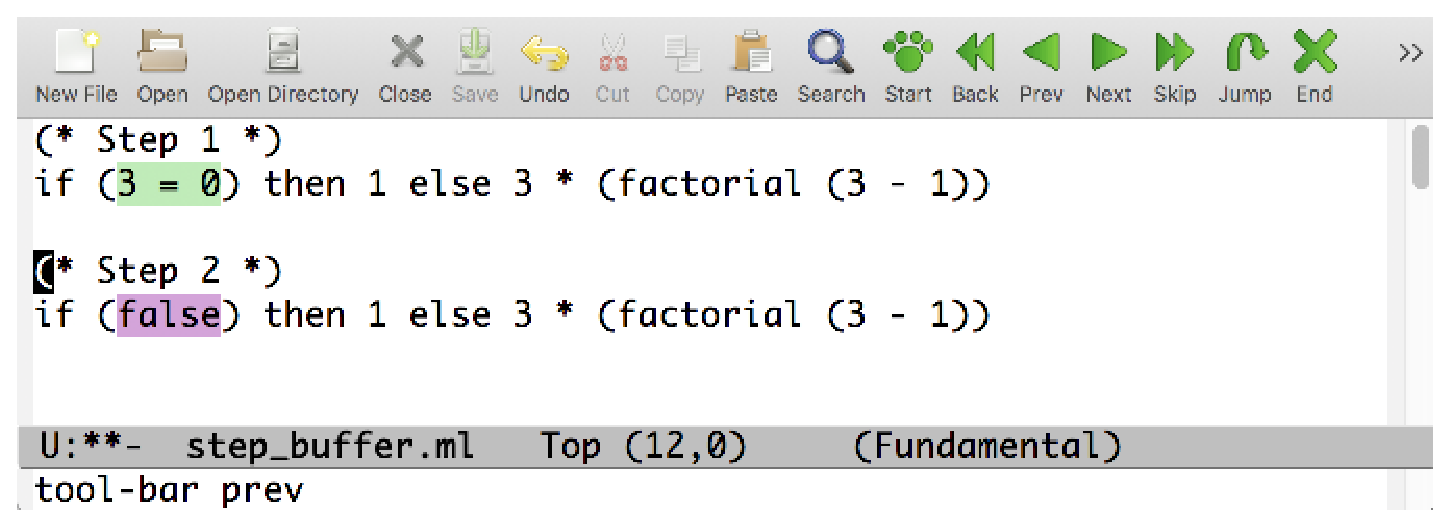
\includegraphics[width=13cm]{1/ocamlfac.eps}
\caption{本研究で実装した OCaml のステッパ}
\label{figure:ocamlfac}
\end{figure}

この中で最も重要なのは 2 つ目、すなわち
入力プログラムを表す構文木を受け取ってステップを表す文字列を出力する関数を作ることである。
それを実現する方法を本論文では 2 種類示している。
そして実装したステッパ (図 \ref{figure:ocamlfac}) を実際に大学の授業において使用し、
学生のプログラム実行ログやアンケートをもとに評価を行った。
その結果、上の 3 つの手順を順番に同期的に行うと
大規模なプログラムをステップ実行する際に 2 つ目の手順に長い時間がかかるため
表示を始めることができないという問題点が発覚した。
その解決のため、1 ステップの実行と表示処理を交互に行うので
ステップ実行処理の終了を待たずに利用できる「incremental なステッパ」を実装した。

\vspace{1cm}
以下に本論文の構成を示す。{\bf 第2章}では、関連研究について述べる。
{\bf 第3章}では、try-with を含む言語を対象にしたステッパの実装方法を説明する。
{\bf 第4章}では、第3章とは別の方法によって algebraic effects
を含む言語を対象にしたステッパの実装方法を説明する。
{\bf 第5章}では、1 ステップずつ実行する incremental なステッパの実装方法を紹介する。
{\bf 第6章}では、プログラミング学習におけるステッパの効果を考察する。
そして{\bf 第7章}で、結論を述べる。
